\documentclass[unicode]{beamer}
\usepackage[T2A]{fontenc}
\usepackage[utf8]{inputenc}
\usepackage[russian]{babel}
\usepackage{cmap}
\usepackage{amssymb,amsfonts,amsmath,mathtext}
\usepackage{beamerthemesplit,graphicx}
% XeTeX packages
\usepackage[cm-default]{fontspec} % or install lmodern and remove cm-default opt
\usepackage{xunicode} % some extra unicode support
\usepackage{xltxtra} % \XeLaTeX macro
\defaultfontfeatures{Scale=MatchLowercase,Mapping=tex-text}
% Setting default fonts
\setromanfont{Charis SIL}
\setsansfont{Charis SIL}
\setmonofont{Charis SIL}

\usepackage{geometry} % Меняем поля страницы
\geometry{left=3mm}% левое поле — не менее 20 мм
\geometry{right=3mm}% правое поле — не менее 10 мм
\geometry{top=0cm}% верхнее поле — не менее 15 мм
\geometry{bottom=0cm}% нижнее поле — не менее 20 мм
\usetheme{Warsaw}
\setbeamerfont{institute}{size=\normalsize}
\graphicspath{{images/}}

\title[Реализация интерфейса приложения HiveMind]{
Реализация интерфейса редактора диаграмм связей HiveMind для Maemo~5
}
\author[Куликов А.\,В.]{Куликов Александр Викторович}
\institute{
Научный руководитель: ст. преподаватель Парамонов~И.\,В.
}

\date{}

\begin{document}
\maketitle
\large

%слайд первый
\begin{frame}
\transwipe[direction=90]
\frametitle{Диаграммы связей}
\begin{figure}[h!] 
\centering
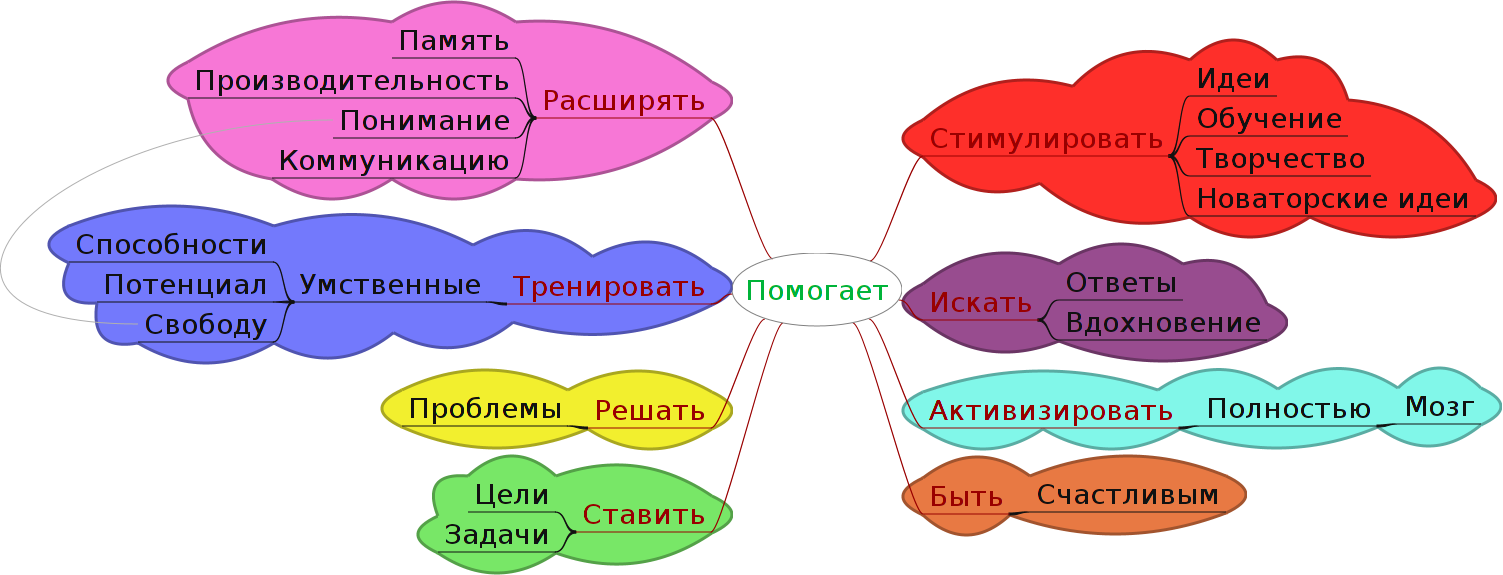
\includegraphics[width=\linewidth]{mind-map} 
\end{figure}
\end{frame}

%второй слайд
\begin{frame}
\transwipe[direction=90]
\frametitle{Проект HiveMind}
\begin{figure}[h!] 
\centering 
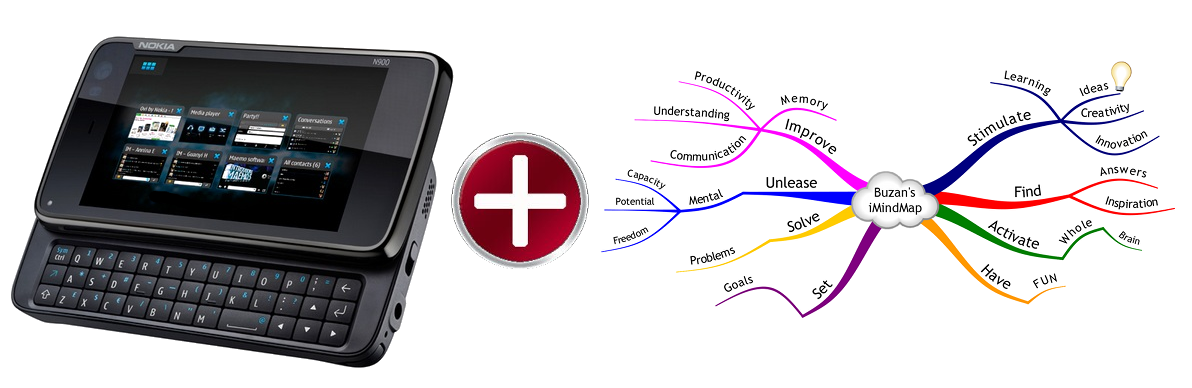
\includegraphics[width=\linewidth]{crossing} 
\end{figure}
Редактор диаграмм связей для мобильных устройств с возможностью совместной работы.
\end{frame}

%третий слайд
\begin{frame}
\transwipe[direction=90]
\frametitle{Постановка задачи}
\begin{itemize}
\item Разработано ранее (другими членами команды):
\begin{itemize}
\item
Классы модели диаграммы связей
\item
Классы для загрузки и сохранения диаграмм связей
\item
Классы для загрузки и сохранения настроек приложения
\end{itemize}
\item
Необходимо реализовать:
\begin{itemize}
\item 
Отображение модели диаграммы связей
\item
Контекстное меню для выбора операций над узлами
\item
Диалог редактирования текста узла
\item
Диалог выбора пиктограмм для узла
\end{itemize}
\end{itemize}
\end{frame}

%четвертый слайд
\begin{frame}
\transwipe[direction=90]
\frametitle{Используемые технологии}
\begin{itemize}
\item
{\textbf{Scratchbox}} --- набор инструментов для кросс-компиляции;
\item
{\textbf{Nokia SDK}} --- универсальный комплект средств разработки приложений для Maemo;
\item
{\textbf{Python}} --- высокоуровневый язык программирования общего назначения;
\item
{\textbf{Qt}} --- кросс-платформенный инструментарий разработки ПО на языке программирования C++;
\item
{\textbf{PySide}} --- привязка языка Python к инструментарию Qt.
\end{itemize}
\end{frame}

%пятый слайд
\begin{frame}
\transwipe[direction=90]
\frametitle{Отображение диаграммы связей}
\begin{figure}[h!] 
\centering 
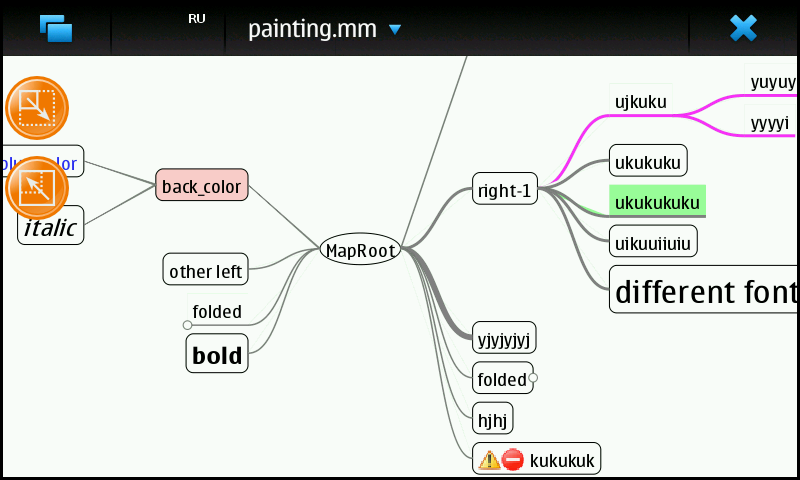
\includegraphics[width=1\linewidth]{main_view} 
\end{figure}
\end{frame}

%шестой слайд
\begin{frame}
\transwipe[direction=90]
\frametitle{Пользователький интерфейса}
\begin{figure}[h!]
\begin{minipage}[h]{0.45\linewidth}
\center{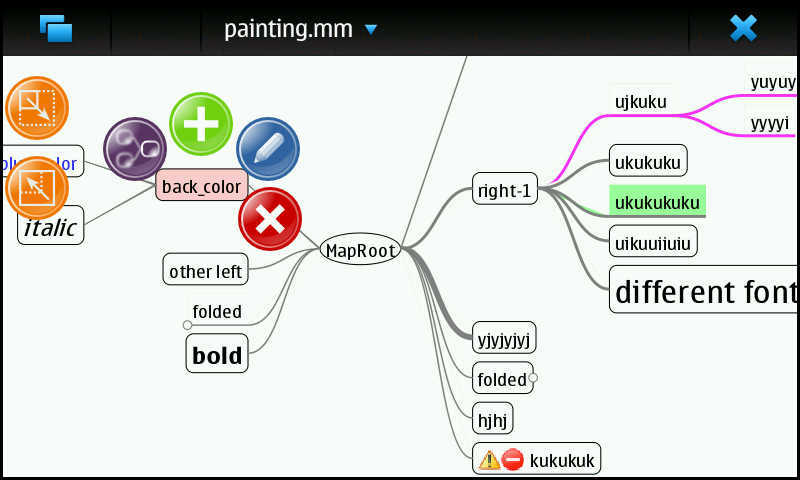
\includegraphics[width=1\linewidth]{context_menu}}
\end{minipage}
\hfill
\begin{minipage}[h]{0.45\linewidth}
\center{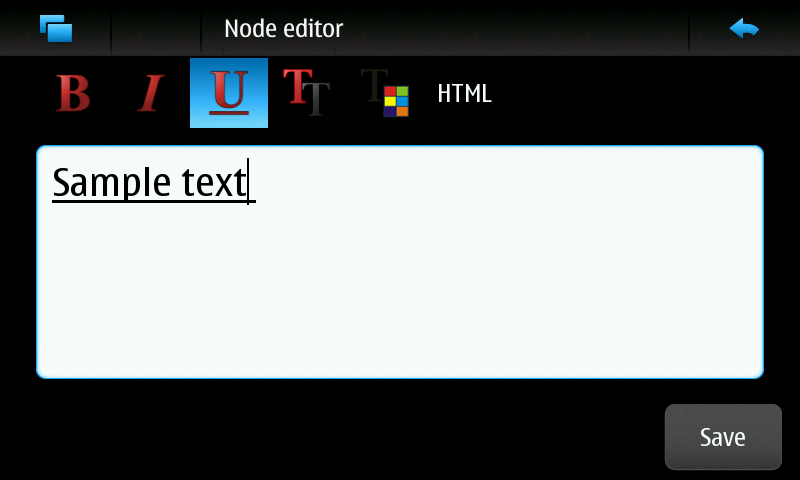
\includegraphics[width=1\linewidth]{text_dialog}}
\end{minipage}
\vfill
\begin{minipage}[h]{0.45\linewidth}
\center{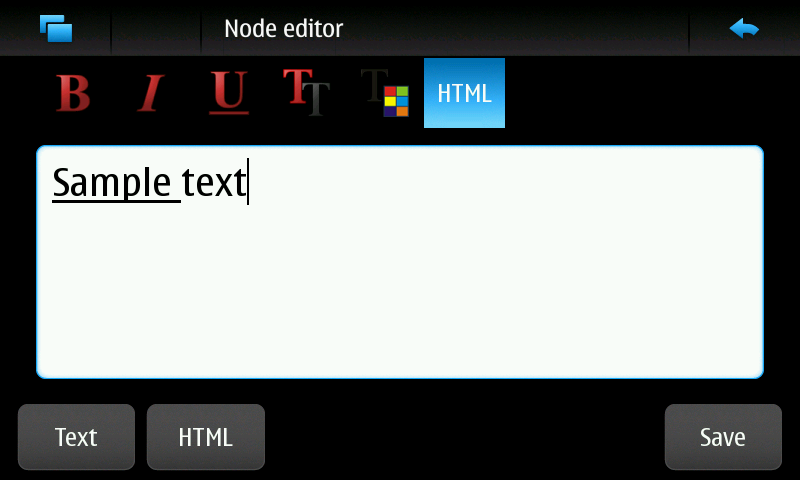
\includegraphics[width=1\linewidth]{html_editor}}
\end{minipage}
\hfill
\begin{minipage}[h]{0.45\linewidth}
\center{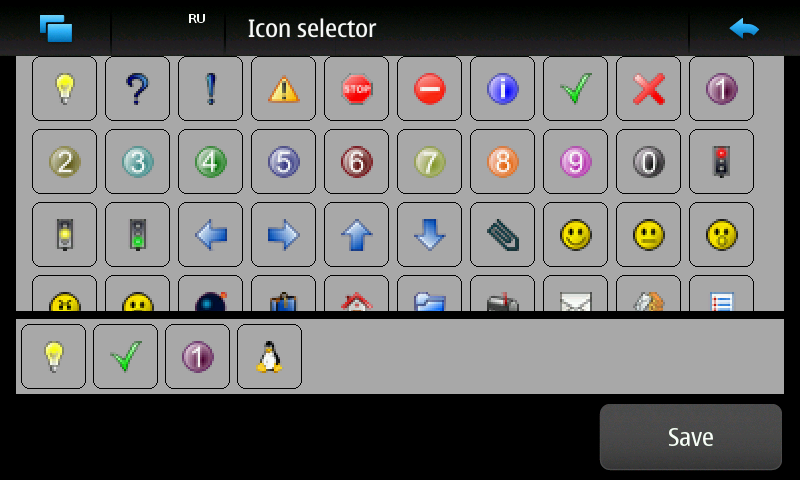
\includegraphics[width=1\linewidth]{icon_selector}}
\end{minipage}
\end{figure}
\end{frame}
\end{document}